\section*{5. Justificación y resumen del stack tecnológico}

El stack tecnológico de este TFG se ha seleccionado para resolver un problema 
híbrido: construir una aplicación web completa (interfaz + API + persistencia) e 
integrar un motor de análisis de datos y Machine Learning con capacidad de 
explicación (XAI). Para ello se adopta una arquitectura cliente‑servidor desacoplada 
y un stack mayoritariamente basado en Python, lo que permite unificar el ciclo de 
vida del dato (obtención $\rightarrow$ limpieza $\rightarrow$ modelado 
$\rightarrow$ predicción $\rightarrow$ explicación) y su exposición a través de 
una API web.

A nivel de principios, las decisiones de tecnología se han guiado por: 
mantenibilidad y modularidad del código, reproducibilidad del entorno, 
viabilidad en el marco temporal de un TFG y escalabilidad razonable. En 
conjunto, el stack se entiende como el conjunto de lenguajes, frameworks, bases 
de datos y herramientas que hacen posible el desarrollo, ejecución y operación 
del sistema.

\subsection*{5.1 Visión general de la arquitectura del sistema}

El sistema se basa en una arquitectura cliente‑servidor desacoplada, estableciendo 
una separación estricta entre frontend, backend/API y motor de procesamiento de 
datos. Esta separación mejora la organización del código y favorece la escalabilidad 
y mantenibilidad: cada capa expone contratos claros y puede evolucionar con menor 
riesgo de efectos colaterales.

\textbf{Capas principales:}

\begin{itemize}
\item \textbf{Capa de presentación (Frontend):} desarrollada con React y Vite. Se 
encarga de la interfaz de usuario, la visualización de datos y la interacción con 
el usuario. Vite se utiliza como servidor de desarrollo y herramienta de build; 
proporciona un flujo moderno con recarga rápida y empaquetado para producción.

\item \textbf{Capa de aplicación / API (Backend):} implementada con Django 5.1.4 + 
Django REST Framework (DRF). Esta capa encapsula la lógica de negocio, la 
autenticación y autorización, la validación de datos, y actúa como puente entre 
la UI y la base de datos/motor de ML. DRF se adopta por su enfoque orientado a 
construir APIs (serializers, viewsets y routers), reduciendo boilerplate y 
estandarizando el diseño de endpoints.

\item \textbf{Capa de procesamiento:} motor especializado en Python que integra 
Pandas/NumPy, librerías de ML (scikit‑learn, XGBoost, LightGBM) y de explicabilidad 
(SHAP). Esta capa puede ejecutarse como módulo interno del backend o como 
componente independiente invocado por tareas programadas, dependiendo del caso de 
uso (entrenamiento offline vs predicción online).

\item \textbf{Capa de persistencia:} gestión de datos relacionales mediante 
PostgreSQL (entorno de producción) y SQLite (entorno de desarrollo). Para 
producción se prioriza PostgreSQL por su robustez y su soporte de transacciones 
(con propiedades ACID), importante para consistencia bajo concurrencia y operaciones 
críticas.
\end{itemize}

\textbf{Comunicación entre capas}

\begin{itemize}
\item Frontend $\leftrightarrow$ Backend/API: comunicación HTTP usando JSON como 
formato principal.

\item Backend $\leftrightarrow$ Persistencia: acceso mediante el ORM de Django, que 
traduce modelos del dominio a tablas relacionales, y permite migraciones y control 
de integridad de forma ordenada.

\item Backend/API $\leftrightarrow$ Motor ML: integración directa en Python para 
minimizar fricción. En ejecución, esto permite que endpoints de predicción llamen 
a un pipeline previamente entrenado y serializado, y devuelvan tanto la predicción 
como elementos de explicación (por ejemplo, top‑features relevantes) cuando proceda.
\end{itemize}

\textbf{Alternativas arquitectónicas consideradas}

Monolito (UI con templates servidor + lógica + procesamiento en una única capa): 
se descartó por el acoplamiento y por dificultar una UI rica y dinámica 
(dashboards, estados complejos) sin mezclar responsabilidades. En un proyecto donde 
el motor de datos/ML evoluciona de forma distinta a la UI, la separación por capas 
reduce deuda técnica y permite trabajar mejor.

Microservicios: aunque es un patrón habitual en sistemas a gran escala, se descartó 
por introducir complejidad operativa no necesaria para el alcance del TFG 
(orquestación, observabilidad distribuida, latencias de red, despliegues 
coordinados). Para los objetivos académicos, la arquitectura desacoplada por capas 
aporta muchas ventajas sin el coste de operación de múltiples servicios.

\begin{figure}[H]
\centering
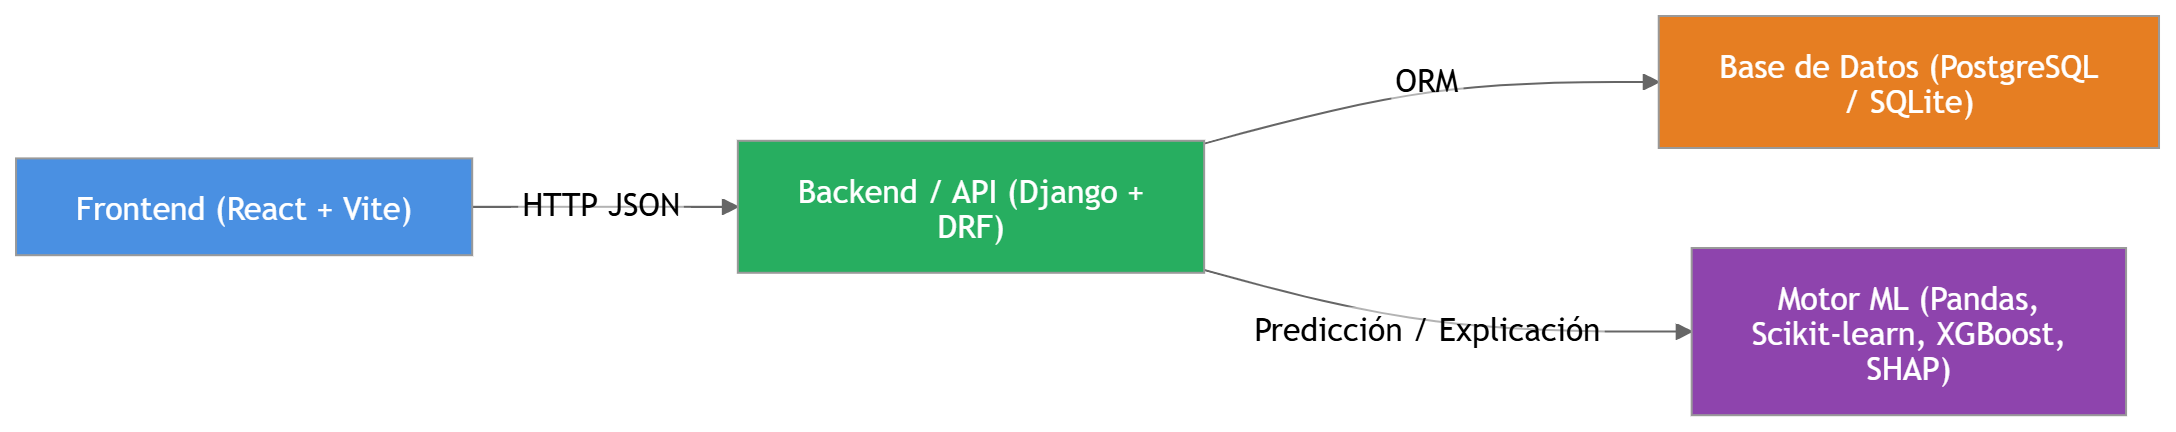
\includegraphics[width=0.58\textwidth]{images/diagrama-resumen.png}
\caption{Diagrama de resumen del stack tecnológico.}\label{fig:stack-resumen}
\end{figure}

\subsection*{5.2 Elección del lenguaje de programación: Python}

La decisión de emplear Python como lenguaje principal se fundamenta en razones técnicas y de 
eficiencia en el desarrollo: el proyecto combina desarrollo web y un componente significativo de 
análisis de datos y Machine Learning. En este contexto, Python destaca por su madurez en el 
ecosistema de ciencia de datos (manipulación, modelado, validación, etc.) y por permitir construir 
el motor predictivo y su integración con la API dentro del mismo entorno.

Además, la elección se apoya en la formación previa: haber trabajado extensamente con Python en el 
grado reduce la curva de aprendizaje y el riesgo técnico, lo cual es relevante en un TFG con 
restricciones de tiempo. Esta continuidad facilita también la reproducibilidad (mismo gestor de 
dependencias y mismas convenciones) y reduce la fragmentación que aparece cuando se mezclan lenguajes 
para piezas íntimamente conectadas.

\textbf{Alternativas consideradas y justificación}

Se analizaron alternativas como Java y JavaScript. Java, especialmente mediante el uso del framework 
Spring Boot, ofrece un entorno empresarial robusto y alto rendimiento, pero presenta mayores barreras 
para integrar flujos completos de Machine Learning, ya que la mayoría de herramientas punteras del 
sector están diseñadas prioritariamente para Python.

Node.js habría permitido unificar el lenguaje en frontend y backend, pero carece de un ecosistema 
maduro en ciencia de datos comparable al de Python. En este proyecto, donde el modelo predictivo es 
un componente central y no accesorio, elegir Python reduce la fricción técnica y permite desarrollar 
todo el ciclo de vida del dato dentro del mismo entorno tecnológico, lo que constituye una ventaja 
estructural significativa.

\subsection*{5.3 Backend: Django 5.1.4 + Django REST Framework}

El backend se implementa con Django 5.1.4 por una combinación de productividad, estructura y 
seguridad. Django proporciona una base sólida para organizar el proyecto (apps, modelos, vistas, 
etc.), y DRF (Django Rest Framework) se incorpora para exponer la funcionalidad mediante una API 
REST. Esto encaja con un frontend desacoplado (React) que consume endpoints, evitando dependencia 
de templates del lado servidor.

Un elemento determinante es el ORM. Modelar entidades del dominio (jugadores, equipos, temporadas, 
partidos, etc.) como modelos declarativos mantiene coherencia con el modelo relacional y facilita 
la evolución del esquema mediante migraciones. Esto reduce el uso de SQL manual en consultas 
repetitivas, disminuye la probabilidad de errores y mantiene un lenguaje común entre lógica de 
negocio y persistencia.

En seguridad, Django incorpora protecciones y buenas prácticas documentadas para mitigar riesgos 
comunes. Por ejemplo, incluye mecanismos integrados para protección contra CSRF (Cross‑Site Request 
Forgery) mediante middleware y herramientas asociadas, especialmente relevante cuando hay sesiones 
o peticiones que modifican estado. Esta base reduce el riesgo de implementar seguridad ``a medida'' 
en un contexto donde lo diferencial del proyecto no es construir un framework de autenticación.

La elección de Django 5.1.4 junto a Django REST Framework responde a la necesidad de construir un 
backend robusto, seguro y altamente modular. Mientras Django proporciona la base estructural (gestión 
de base de datos, seguridad y administración), DRF se incorpora para transformar estas capacidades 
en una API RESTful que sirve como el núcleo del sistema, promoviendo las buenas prácticas en el 
desarrollo software.

Además, el sistema de autenticación y autorización integrado de Django (usuarios, permisos, grupos) 
permite gestionar control de acceso con componentes maduros. En un proyecto académico, esto aporta 
valor porque focaliza el esfuerzo en el dominio deportivo y el componente predictivo.

\textbf{Alternativas consideradas y justificación}

Flask: ofrece flexibilidad, pero obliga a ensamblar manualmente múltiples piezas (auth, estructura, 
admin, convenciones), lo que aumenta el tiempo de desarrollo y la probabilidad de inconsistencias.

FastAPI: destaca por rendimiento, tipado y documentación automática; aun así, Django aporta una 
solución más integral cuando hay fuerte componente relacional, gestión de usuarios y necesidad de 
herramientas integradas (admin/ORM/migraciones) con alta madurez.

Spring Boot / Express: la principal desventaja en este proyecto sería la pérdida de integración 
directa con el stack de ML en Python o la necesidad de introducir servicios adicionales para el 
motor predictivo.

\subsection*{5.4 Persistencia y base de datos: SQLite y PostgreSQL}

Durante la fase de desarrollo se ha utilizado SQLite por su simplicidad operativa: permite comenzar 
a trabajar con rapidez, no requiere desplegar servicios adicionales y se integra de forma inmediata 
con Django, lo que resulta especialmente útil en etapas tempranas de prototipado y pruebas. No 
obstante, para el entorno de producción se realizará la migración a PostgreSQL, con el objetivo de 
disponer de una solución más robusta y preparada para crecer en volumen de datos y número de 
usuarios.

PostgreSQL es un sistema gestor de bases de datos relacional ampliamente adoptado en entornos 
profesionales y considerado una tecnología muy estandarizada, lo que facilita su integración con 
herramientas del ecosistema y reduce riesgos de mantenimiento a largo plazo. Además, ofrece garantías 
transaccionales ACID, aportando fiabilidad en operaciones críticas y consistencia del dato incluso 
ante fallos o ejecuciones concurrentes.

PostgreSQL también destaca por su buen comportamiento en escenarios con acceso simultáneo a datos, 
algo habitual cuando el sistema empieza a recibir varias peticiones a la vez (consultas desde la UI, 
escrituras de nuevas predicciones, etc.). Esta capacidad de gestionar concurrencia de forma eficiente 
permite mantener una experiencia de uso más estable y reduce problemas derivados de bloqueos y esperas 
en la base de datos conforme aumenta la carga. Por ello, la migración a PostgreSQL se plantea como 
una elección orientada a producción: una base de datos relacional madura y estandarizada, preparada 
para soportar crecimiento y operaciones críticas con garantías consistentes.

\textbf{Alternativas consideradas y justificación}

Se consideraron alternativas como MySQL o bases de datos NoSQL. MySQL ofrece prestaciones similares; 
sin embargo, PostgreSQL destaca por su mayor cumplimiento de los estándares SQL y por sus capacidades 
avanzadas de indexación y gestión de consultas complejas. Por su parte, soluciones NoSQL como MongoDB 
podrían haber ofrecido un mayor rendimiento en determinados escenarios de alta escalabilidad o grandes 
volúmenes de datos no estructurados. No obstante, su adopción implicaba una curva de aprendizaje 
adicional y un cambio en el modelo de diseño orientado a documentos que no resultaba óptimo para un 
sistema con fuerte componente relacional y consultas estructuradas complejas.

En este contexto, la elección de PostgreSQL permitió mantener coherencia con el modelo de datos 
planteado, reducir la complejidad técnica y optimizar el tiempo de desarrollo sin comprometer el 
rendimiento necesario para el proyecto.

\subsection*{5.5 Procesamiento de datos y Machine Learning}

El proyecto incorpora un pipeline de datos completo que no se limita a entrenar un modelo: incluye 
ingesta, limpieza, construcción de features, validación, evaluación e interpretabilidad.

\subsubsection*{5.5.1 Preprocesado y ETL (Extract, Transform and Load)}

Se emplean Pandas y NumPy para:

\begin{itemize}
\item Limpieza y normalización (tipos, formatos de fecha, estandarización de nombres).
\item Tratamiento de nulos y outliers.
\item Codificación de variables categóricas y construcción de datasets finales.
\item Generación de features a partir de histórico (medias móviles, acumulados, forma reciente, 
local/visitante, etc.), cuidando que las features respeten la causalidad temporal (evitar 
``data leakage'').
\end{itemize}

El resultado del ETL es un dataset donde filas representan un hecho (p. ej., equipo en jornada, 
jugador en partido) y columnas representan variables. Este enfoque tabular es coherente con la 
mayoría de datos deportivos agregados, donde la señal predictiva suele estar en combinaciones de 
variables independientes.

\subsubsection*{5.5.2 Modelado (scikit‑learn, XGBoost, LightGBM)}

Se utiliza scikit‑learn para evaluación y validación (splits, métricas, pipelines y comparación de 
enfoques). Además, se exploran modelos basados en árboles y gradient boosting (XGBoost y LightGBM), 
especialmente competitivos en dominios tabulares por su capacidad de capturar no linealidades e 
interacciones con buen coste computacional.

La elección de boosting se justifica por:

\begin{itemize}
\item Buen rendimiento en tabular con variables heterogéneas.
\item Estabilidad razonable con datasets medianos.
\item Menor coste de ingeniería comparado con deep learning para este tipo de dato.
\end{itemize}

\subsubsection*{5.5.3 Interpretabilidad (XAI con SHAP)}

La interpretabilidad se aborda con SHAP para generar explicaciones:

\begin{itemize}
\item \textbf{Globales:} identificar qué variables influyen más de forma general en el modelo.
\item \textbf{Locales:} justificar una predicción individual descomponiéndola en contribuciones por 
feature.
\end{itemize}

Esto añade valor académico y práctico: el sistema no se limita a una salida numérica, sino que ofrece 
una narrativa técnica de ``por qué'' se produce la predicción, reduciendo el carácter de caja negra y 
facilitando el análisis de errores.

\textbf{Alternativas consideradas y justificación}

Se evalúa deep learning (TensorFlow/PyTorch), pero para datos tabulares suele 
requerir más ajuste, más datos y mayor coste de entrenamiento para obtener mejoras 
no garantizadas frente a boosting. Dado el alcance del TFG, se prioriza un enfoque 
más eficiente y explicable.

\subsubsection*{5.5.4 Serialización e integración del modelo predictivo (Pickle)}

Para materializar la conexión entre la fase de entrenamiento y el entorno de 
operación, se hace uso del módulo pickle de Python. Una vez que el pipeline de 
preprocesamiento y los modelos predictivos han sido entrenados y validados, el 
objeto resultante se serializa y se exporta como un archivo binario (.pkl).

En tiempo de ejecución, el backend de Django carga este artefacto en memoria al 
inicializar la aplicación o al instanciar la clase predictiva. Esta estrategia 
permite que los endpoints de la API realicen predicciones invocando al modelo ya 
ajustado, sin necesidad de retener en el servidor los datos de entrenamiento ni 
recalcular pesos. De esta forma, se garantiza una latencia baja en la respuesta 
HTTP y se mantiene una separación estricta entre el ciclo de entrenamiento 
(offline) y el de inferencia (online).

\subsection*{5.6 Obtención de datos y scraping}

El proyecto requiere recopilar información deportiva desde fuentes heterogéneas, por lo que se adopta 
una estrategia híbrida de ingesta. En la práctica, muchas fuentes presentan limitaciones: APIs 
incompletas, restricciones de uso, cambios de condiciones o modelos de pago, por lo que combinar 
técnicas permite maximizar cobertura manteniendo viabilidad.

\subsubsection*{5.6.1 Descarga de CSVs con cuotas (Football‑Data.co.uk)}

Una fuente clave de cuotas de apuestas son los ficheros CSV públicos de Football‑Data.co.uk 
(SP1.csv), que ofrece enlaces de descarga histórica para España. Estos CSVs se integran en el 
pipeline como datasets de entrada: se descargan y se normalizan para cruzarlos con el resto de 
tablas del dominio.

\subsubsection*{5.6.2 Consumo de APIs y evaluación de librerías}

A lo largo del desarrollo se exploran distintas APIs/librerías de datos deportivos (por ejemplo 
statsbomb, soccerdata), algunas finalmente descartadas por limitaciones prácticas (cobertura, 
estabilidad, compatibilidad con el dataset objetivo). Este trabajo forma parte de la ingeniería de 
datos: evaluar fuentes, comparar consistencia temporal y decidir qué fuentes cumplen requisitos 
mínimos (completitud, actualización, integrabilidad).

Además, se utiliza REST Countries para enriquecer la UI con información contextual (por ejemplo 
banderas/países) sin mantener un dataset propio cuando no es parte nuclear del problema.

\subsubsection*{5.6.3 Scraping: requests + parsing HTML}

Dadas las limitaciones con las APIs, en la mayoría de casos se recurre a scraping con requests y 
parsing con BeautifulSoup4 con lxml. Esta decisión permite mantener viabilidad económica y cobertura 
de datos, asumiendo el coste técnico de:

\begin{itemize}
\item Normalizar formatos heterogéneos.
\item Diseñar extractores robustos.
\item Mitigar roturas ante cambios de HTML.
\end{itemize}

\subsection*{5.7 Frontend con React y Vite}

La capa de presentación se desarrolla con React por su enfoque basado en componentes, idóneo para 
dashboards y vistas con alta reutilización (tarjetas de jugadores, tablas, filtros, gráficos, 
paneles de explicación). Se utiliza Vite como herramienta de build y servidor de desarrollo, 
mejorando significativamente la experiencia de desarrollo en comparación con herramientas 
tradicionales más pesadas.

\subsubsection*{5.7.1 Desacoplamiento respecto al servidor}

Inicialmente se valora usar templates del lado servidor (Django templates), lo cual habría 
simplificado la arquitectura a corto plazo. Sin embargo, se opta por un frontend desacoplado para 
mantener separación de responsabilidades y permitir una evolución más flexible: rutas del cliente, 
estados complejos y consumo de API de forma limpia.

\subsubsection*{5.7.2 Base estructural: adaptación de React Petclinic}

El proyecto toma como base estructural React Petclinic, del cual se elimina toda la interfaz y 
entidades, manteniendo únicamente el ``esqueleto funcional'' para adaptarlo al dominio deportivo. 
Esta decisión acelera la construcción inicial (estructura de componentes, navegación, etc.) y permite 
centrar más esfuerzo en las partes diferenciales (datos, predicción, explicaciones y UX de análisis).

\textbf{Alternativas consideradas y justificación}

Angular: muy completo y estructurado, pero con mayor curva de aprendizaje y sobrecarga conceptual 
para el alcance del TFG.

Vue: productivo y simple, pero React ofrece adopción industrial muy extendida y un ecosistema enorme 
para visualización y gestión de estado.

Templates del servidor: más sencillo al principio, pero limita escalabilidad de UI y mezcla 
responsabilidades, complicando la evolución hacia un cliente rico.

\subsection*{5.8 APIs y otras herramientas de soporte (búsqueda, matching, enriquecimiento)}

Además de la API principal (DRF), se incorporan herramientas complementarias para resolver 
necesidades de producto y de explotación del dato:

\textbf{Fuzzy matching:} se incorpora para resolver pequeñas variaciones textuales (nombre real vs 
apodos, diferencias ortográficas) al conciliar entidades entre fuentes. Esto es habitual cuando se 
combinan datasets externos y scraping.

\textbf{Opensearch:} se emplea como motor de búsqueda para habilitar consultas rápidas sobre campos 
de texto (nombres de jugadores/equipos). Opensearch construye un índice invertido a partir del 
texto analizado, lo que permite búsquedas full‑text eficientes y ranking por relevancia.

Este conjunto de herramientas se justifica por un objetivo práctico: mejorar la experiencia de usuario 
(búsquedas rápidas, navegación fluida) y reducir fricción en la integración de datos (matching y 
normalización).

\subsection*{5.9 Entorno de desarrollo, despliegue y calidad de software}

El proyecto adopta herramientas estándar para garantizar reproducibilidad, facilitar el desarrollo 
y sostener calidad de software. Aunque el alcance sea académico, estas decisiones aproximan el 
trabajo a prácticas profesionales y reducen riesgos técnicos.

\subsubsection*{5.9.1 Gestión de Entornos Virtuales y Dependencias}

Dado que el proyecto utiliza una gran cantidad de librerías con versiones específicas (especialmente 
en el stack de Machine Learning), se ha optado por el uso de entornos virtuales mediante venv 
(Python Virtual Environments).

\textbf{Aislamiento:} Esta técnica permite que las dependencias del proyecto residan en un directorio 
local, evitando conflictos con las librerías globales del sistema operativo.

\textbf{Pip y requirements.txt:} La gestión de paquetes se realiza a través de pip. Para asegurar que 
el motor de ML y el backend de Django funcionen correctamente en cualquier máquina, se mantiene un 
archivo requirements.txt actualizado. Este archivo actúa como el ``contrato de dependencias'' del 
sistema, permitiendo la instalación masiva de las versiones exactas necesarias mediante un solo 
comando. Puede ser generado automáticamente con diferentes herramientas, lo que disminuye en gran 
medida la complejidad de su elaboración.

\subsubsection*{5.9.2 Contenedores y orquestación: viabilidad de Docker}

Se ha implementado una arquitectura basada en contenedores utilizando Docker, lo que permite aislar 
cada componente del sistema en un entorno controlado. Para la gestión de estos servicios, se emplea 
Docker Compose, actuando como el orquestador que define y arranca los cuatro nodos principales que 
conforman la aplicación:

\begin{itemize}
\item \textbf{Backend (API):} Contenedor basado en Python 3.12 que aloja la lógica de Django y el 
motor de Machine Learning.

\item \textbf{Frontend (UI):} Contenedor que sirve la aplicación React, optimizada tras el proceso 
de build de Vite.

\item \textbf{Persistencia (PostgreSQL):} Servicio dedicado para la base de datos relacional, 
asegurando el almacenamiento persistente mediante volúmenes de Docker.

\item \textbf{Motor de Búsqueda (OpenSearch):} Nodo independiente para la indexación y búsqueda 
avanzada de datos, garantizando que los procesos de búsqueda intensiva no penalicen el rendimiento 
de la base de datos principal o no afecte al no estar disponible.
\end{itemize}

\textbf{Ventajas de este enfoque:}

\begin{itemize}
\item \textbf{Consistencia entre entornos:} Se elimina el problema de ``funciona en mi máquina'', ya 
que el entorno de desarrollo es idéntico al de producción.

\item \textbf{Aislamiento de dependencias:} Cada servicio tiene sus propias librerías y 
configuraciones (por ejemplo, el stack de ML en el backend no interfiere con el motor de búsqueda).

\item \textbf{Escalabilidad y portabilidad:} La arquitectura está preparada para ser desplegada en 
cualquier proveedor de nube (AWS, Azure, Google Cloud, etc.) mediante un único comando, lo que reduce 
drásticamente la complejidad operativa.
\end{itemize}

\subsubsection*{5.9.3 Control de versiones, planificación y control de calidad}

\textbf{Control de versiones:} GitHub.

\textbf{Planificación temporal:} Microsoft Project.

\textbf{Registro de horas:} Clockify.

\textbf{Calidad:} SonarQube para análisis estático.


\begin{figure}[H]
\centering
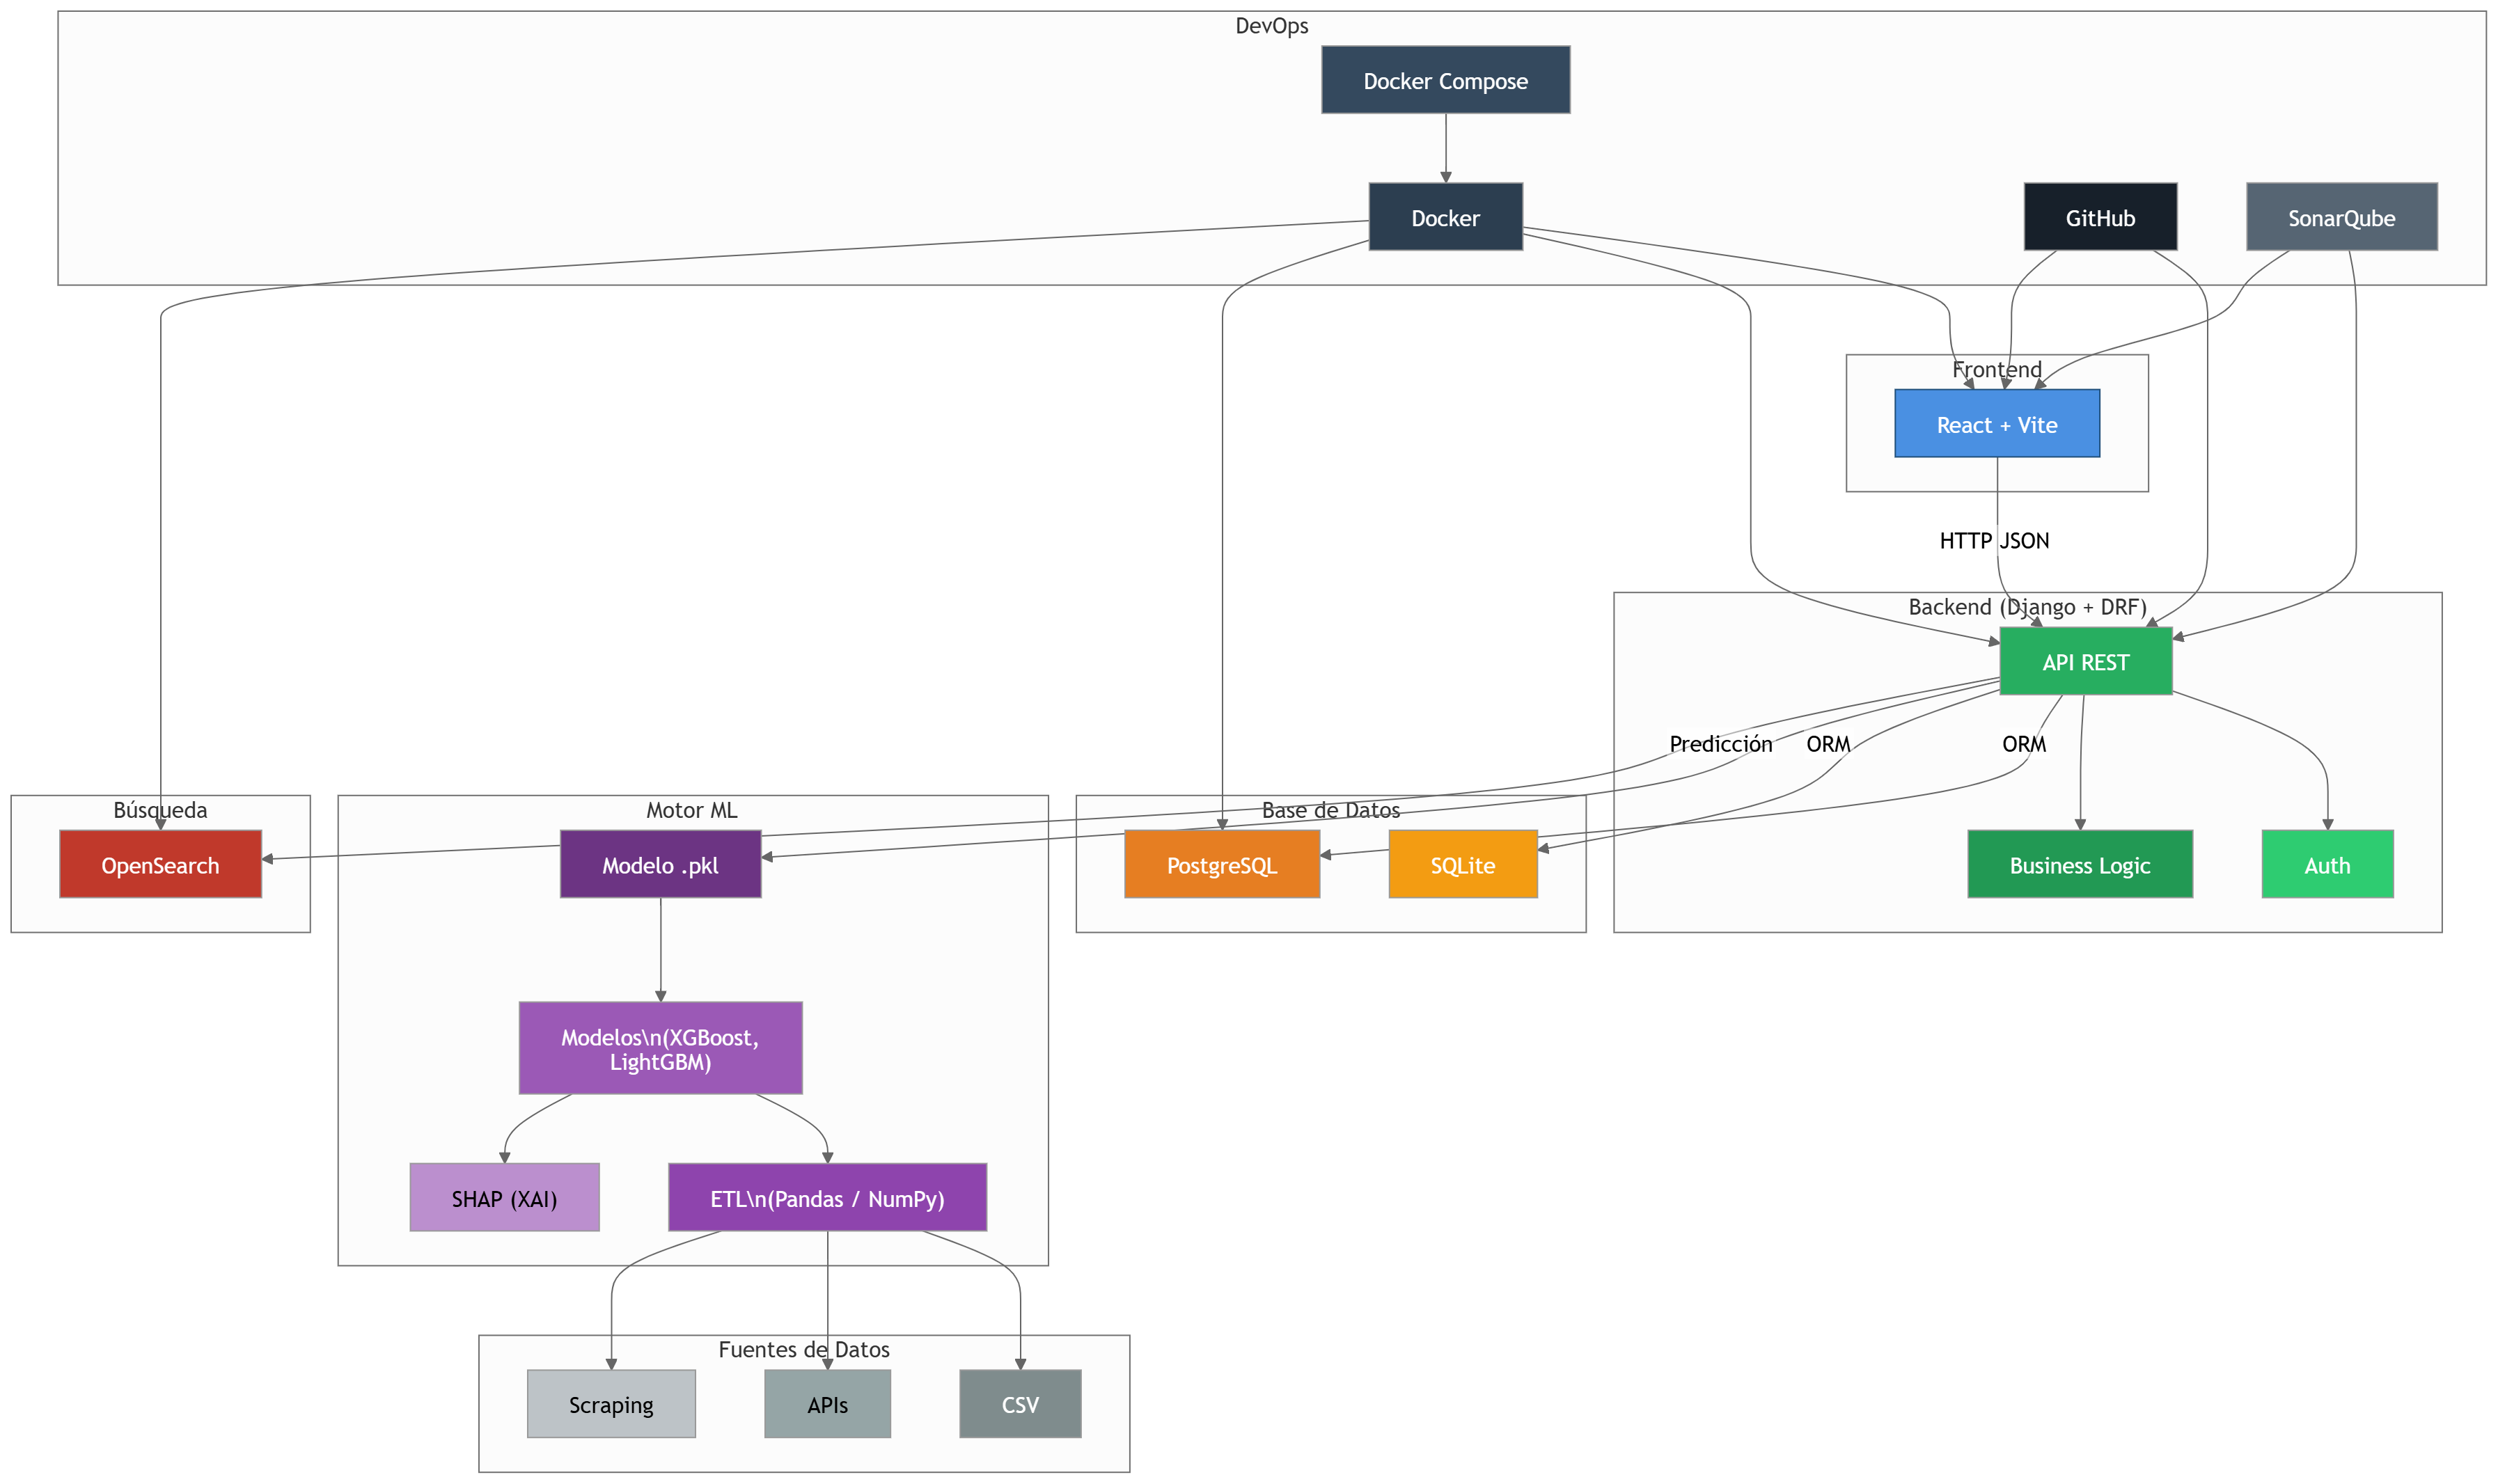
\includegraphics[width=1\textwidth]{images/arquitectura-completa.png}
\caption{Estructura del sistema y comunicación entre sus capas.}\label{fig:arquitectura-sistema}
\end{figure}